% ===================== Executive summary: two pages, visual first =====================
\newgeometry{left=22mm,right=22mm,top=15mm,bottom=17mm}
\fancypagestyle{execfoot}{\fancyhf{}\renewcommand{\headrulewidth}{0pt}\renewcommand{\headrule}{}\fancyfoot[C]{\small\sffamily\color{muted}\thepage}}
\thispagestyle{empty}\phantomsection\addcontentsline{toc}{section}{Executive summary}
\markboth{Executive summary}{Executive summary}
\definecolor{claycol}{HTML}{EFE4D6}
\definecolor{sandcol}{HTML}{DCE9F8}
\definecolor{deepcol}{HTML}{E3E7EA}
% section label with a pointer to the full section
\newcommand{\xhead}[2]{\par\vspace{2.2mm}\noindent
  {\sffamily\bfseries\small\color{accent}\MakeUppercase{#1}}\hfill{\sffamily\scriptsize\color{muted}#2}\\[-7pt]
  {\color{line}\rule{\linewidth}{0.5pt}}\par\vspace{0.6mm}}
\newcommand{\xyes}{\textcolor{green}{\large\checkmark}}
\newcommand{\xno}{\textcolor{line}{\rule[2pt]{9pt}{1.2pt}}}
\newcommand{\xpart}{\textcolor{muted}{\sffamily\scriptsize partly}}
\tcbset{tile/.style={enhanced,colback=#1,colframe=#1,boxrule=0pt,arc=2pt,left=7pt,right=7pt,top=6pt,bottom=6pt,
  fontupper=\sffamily\footnotesize\raggedright}}
\newcommand{\tilebig}[2]{{\sffamily\bfseries\fontsize{19}{21}\selectfont\color{#1}#2}\\[2pt]}

\begin{center}
{\sffamily\scriptsize\color{muted} ASEAN Geospatial Challenge 2027 \textbullet\ National Level: Indonesia \textbullet\ working document, 16 November 2026}\\[3mm]
{\sffamily\bfseries\fontsize{24}{27}\selectfont\color{ink} Groundwater Audit from Space}\\[2mm]
{\sffamily\large\color{accent} Tracing land subsidence in Semarang--Demak back to the pumping that causes it}
\end{center}
\vspace{-1mm}

\begin{tcolorbox}[enhanced,colback=accent,colframe=accent,boxrule=0pt,arc=2pt,left=10pt,right=10pt,top=7pt,bottom=7pt]
\sffamily\color{white}\textbf{Executive summary.} Satellites already show \emph{where} the coast of Central Java
is sinking. This project works out \emph{which pumping causes it, and how much}: a ranked list of
groundwater extraction hot spots, each with a volume and an error bar, made without a well registry.
\end{tcolorbox}

% ---------------------------------------------------------------- PROBLEM
\xhead{The problem}{Sections \ref{sec:problem}--\ref{sec:area}}
\begin{tcbraster}[raster columns=3,raster equal height,raster column skip=3mm,raster before skip=1mm,raster after skip=0mm]
\begin{tcolorbox}[tile=warmsoft]
\tilebig{warm}{14\,cm a year}
The fastest sinking measured in Semarang and Demak, 2020--2023 \cite{janur2025}. Tidal floods (\emph{rob}) keep getting worse.
\end{tcolorbox}
\begin{tcolorbox}[tile=warmsoft]
\tilebig{warm}{2010}
The last year with usable well records. By then more than 1,000 deep wells were pumping
\cite{lo2022,putranto2016}.
\end{tcolorbox}
\begin{tcolorbox}[tile=warmsoft]
\tilebig{warm}{Which wells?}
Permits exist, but nobody can say which pumping does the damage. Inspectors have no list to
start from.
\end{tcolorbox}
\end{tcbraster}

% ---------------------------------------------------------------- IDEA
\xhead{The idea: pumping leaves a fingerprint on the ground}{Section \ref{sec:physics}}
\noindent
\begin{minipage}[c]{0.59\linewidth}
\begin{tikzpicture}[x=1cm,y=1.22cm,font=\sffamily\scriptsize]
  \def\surf{(0,3.5) .. controls (2.2,3.5) and (3.0,3.1) .. (4.3,3.1) .. controls (5.6,3.1) and (6.4,3.5) .. (8.6,3.5) -- (9.6,3.5)}
  % layers
  \fill[deepcol] (0,0) rectangle (9.6,0.5);
  \fill[sandcol] (0,0.5) rectangle (9.6,1.7);
  \fill[claycol] (0,1.7) -- \surf -- (9.6,1.7) -- cycle;
  % old and new surface
  \draw[muted,dash pattern=on 2pt off 2pt,line width=0.4pt] (0,3.5) -- (9.6,3.5);
  \draw[ink,line width=0.9pt] \surf;
  % layer names
  \node[anchor=east,text=muted] at (9.5,2.17) {clay};
  \node[anchor=east,text=muted] at (9.5,0.95) {aquifer: sand and water};
  % pressure level before and after
  \draw[accent,dash pattern=on 2pt off 2pt,line width=0.5pt] (0,2.72) -- (9.6,2.72);
  \draw[accent,line width=1.1pt] (0,2.66) .. controls (2.6,2.62) and (3.7,2.3) .. (4.3,1.0)
       .. controls (4.9,2.3) and (6.0,2.62) .. (9.6,2.66);
  \node[anchor=west,text=accent] at (0.1,2.93) {pressure before pumping};
  % well and factory
  \draw[ink,line width=1.2pt] (4.3,3.1) -- (4.3,0.85);
  \fill[ink] (4.0,3.1) rectangle (4.8,3.38);
  \fill[ink] (4.0,3.38) -- (4.0,3.58) -- (4.27,3.38) -- (4.27,3.58) -- (4.54,3.38) -- (4.54,3.58) -- (4.8,3.38) -- cycle;
  \draw[accent,-{Stealth[length=4pt]},line width=0.9pt] (4.4,3.72) -- (4.4,4.15);
  % compaction arrows
  \foreach \x in {2.3,2.8,5.9,6.4} \draw[warm,-{Stealth[length=3pt]},line width=0.8pt] (\x,2.38) -- (\x,1.95);
  % sinking arrow
  \draw[ink,-{Stealth[length=3pt]},line width=0.7pt] (5.75,3.5) -- (5.75,3.24);
  % satellites
  \foreach \sx/\tx in {1.3/3.2,8.3/5.4}{
    \draw[muted,dash pattern=on 1.5pt off 1.5pt,line width=0.4pt] (\sx,5.1) -- (\tx,3.25);
    \fill[ink] (\sx-0.16,5.03) rectangle (\sx+0.16,5.23);
    \fill[accent] (\sx-0.62,5.08) rectangle (\sx-0.2,5.18);
    \fill[accent] (\sx+0.2,5.08) rectangle (\sx+0.62,5.18);
  }
  \node[text=muted] at (4.8,5.13) {radar satellite, two viewing directions};
  % step tags
  \node[anchor=west,text=ink] at (4.52,4.0) {\textcolor{accent}{\cir{1}} pumping};
  \node[anchor=west,text=accent] at (4.75,1.2) {\cir{2} pressure cone};
  \node[anchor=west,text=warm] at (0.1,2.17) {\cir{3} clay compacts};
  \node[anchor=west,text=ink] at (5.9,3.74) {\cir{4} ground sinks};
\end{tikzpicture}
\end{minipage}\hfill
\begin{minipage}[c]{0.37\linewidth}\sffamily\footnotesize\raggedright
\textcolor{accent}{\cir{1}} A deep well pumps water out.\\[2.5pt]
\textcolor{accent}{\cir{2}} Water pressure falls in a cone several kilometres wide.\\[2.5pt]
\textcolor{warm}{\cir{3}} Clay drains and compacts. Most of this is permanent.\\[2.5pt]
\cir{4} The ground sinks in the same cone shape. Radar measures it from space.\\[5pt]
\begin{tcolorbox}[tile=greensoft,left=6pt,right=6pt,top=5pt,bottom=5pt]
\textbf{\color{green}We read the chain backwards}, from \cir{4} to \cir{1}. The shape of each
bowl tells us where the pumping sits and how much storage is lost there.
\end{tcolorbox}
\end{minipage}

% ---------------------------------------------------------------- SOLUTION
\xhead{The solution: from a sinking map to an audit list}{Section \ref{sec:exp}}
\begin{center}
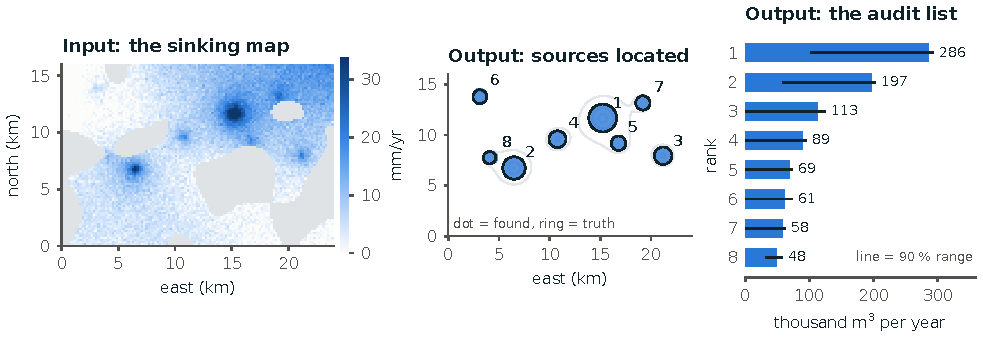
\includegraphics[width=\linewidth]{fig/exec_solution.pdf}
\end{center}
\vspace{-3mm}
{\sffamily\scriptsize\color{muted} One of \nScen\ simulated test maps, with the noise and data gaps of real radar. Eight sources
were hidden; the method found all eight and ranked them. Volume means storage lost by the aquifer, a
lower bound on water pumped. A run on real Semarang data is the next step (Section~\ref{sec:spike}).\par}

\clearpage\thispagestyle{execfoot}
% ======================================================================= PAGE 2
% ---------------------------------------------------------------- METHOD
\xhead{The method in three moves}{Sections \ref{sec:method}--\ref{sec:rigour}}
\noindent
\begin{tikzpicture}[font=\sffamily\footnotesize]
  \tikzset{card/.style={rounded corners=2pt,text width=46.5mm,minimum height=28mm,align=flush left,inner sep=6pt,anchor=north west}}
  \node[card,fill=accentsoft] (a) at (0,0) {%
    {\bfseries\color{accent}1\quad Measure}\hfill\M{1}--\M{3}\\[3pt]
    Ten years of Sentinel-1 radar from \textbf{two directions}. Result: vertical motion for every
    100\,m pixel, tied to BIG's own GNSS stations.};
  \node[card,fill=greensoft] (b) at (55.5mm,0) {%
    {\bfseries\color{green}2\quad Separate}\hfill\M{4}--\M{5}\\[3pt]
    Remove what is \textbf{not pumping}: natural clay settling, building load, seasons. Learned
    by boosted trees on quiet pixels only.};
  \node[card,fill=warmsoft] (c) at (111mm,0) {%
    {\bfseries\color{warm}3\quad Invert}\hfill\M{6}--\M{9}\\[3pt]
    Find the \textbf{fewest pumping cones} that explain the rest. A bootstrap gives every source a
    range and a stability score.};
  \draw[arr,line width=0.9pt] ($(a.east)+(0.5mm,0)$) -- ($(b.west)+(-0.5mm,0)$);
  \draw[arr,line width=0.9pt] ($(b.east)+(0.5mm,0)$) -- ($(c.west)+(-0.5mm,0)$);
\end{tikzpicture}

\vspace{1mm}
{\sffamily\footnotesize\color{ink}\textbf{Why it is rigorous.} A physics model sits inside the learning step, so every
number has a unit. Splits are spatial blocks, never random pixels. Each learned part has a baseline
to beat and a pass mark set in advance (\V{1}--\V{7}).\par}

% ---------------------------------------------------------------- EVIDENCE
\xhead{The evidence so far}{Section \ref{sec:exp}}
\noindent
\begin{minipage}[t]{0.56\linewidth}\vspace{0pt}
\begin{tikzpicture}[x=0.42mm,y=1mm,font=\sffamily\scriptsize]
  % x from 0 to 100 (%), label column to the left
  \def\barrow#1#2#3#4{% y, label, recall, precision
    \node[anchor=east,align=right,text=ink] at (-3,#1+2.6) {#2};
    \fill[accent!85] (0,#1+3.0) rectangle (#3,#1+6.0);
    \fill[warm!80] (0,#1-0.6) rectangle (#4,#1+2.4);
    \node[anchor=west,text=ink] at (#3,#1+4.5) {#3\,\%};
    \node[anchor=west,text=ink] at (#4,#1+0.9) {#4\,\%};
  }
  \draw[line] (0,-2.0) -- (0,27.5);
  \barrow{20}{Add up each bowl\\by hand}{\boRecall}{\boPrecision}
  \barrow{10}{Smooth inversion\\(closest earlier work)}{\smRecall}{\smPrecision}
  \barrow{0}{\textbf{Sparse inversion}\\\textbf{(this project)}}{\calRecall}{\calPrecision}
  \fill[accent!85] (0,-7.5) rectangle (4,-5.5); \node[anchor=west] at (5,-6.5) {sources found};
  \fill[warm!80] (52,-7.5) rectangle (56,-5.5); \node[anchor=west] at (57,-6.5) {detections that are real};
\end{tikzpicture}
\end{minipage}\hfill
\begin{minipage}[t]{0.41\linewidth}\vspace{0pt}\sffamily\footnotesize\raggedright
\textbf{\nScen\ simulated maps, \nTrue\ hidden sources.} Only the sparse inversion both finds the
sources and avoids false alarms.\\[5pt]
\begin{tabular}{@{}>{\bfseries\fontsize{15}{17}\selectfont\color{accent}}r@{\hspace{7pt}}L{43mm}@{}}
\calMedErr\,\% & median volume error, when the cone width is known\\[2pt]
\calLoc\,m & median position error\\[2pt]
\calCover\,\% & of true volumes fall inside the stated 90\,\% range\\
\end{tabular}
\end{minipage}

\vspace{1mm}
\begin{tcolorbox}[tile=warmsoft,left=8pt,right=8pt,top=4pt,bottom=3pt]
\begin{minipage}[c]{0.47\linewidth}\raggedright
\textbf{\color{warm}The honest limit: one number we cannot see from space.}
Volumes depend on the width of a pumping cone. Guess it wrong and every volume shifts together.
The \emph{order} of the list barely moves.
\end{minipage}\hfill
\begin{minipage}[c]{0.50\linewidth}
\begin{tikzpicture}[x=20mm,y=1mm,font=\sffamily\scriptsize]
  \node[anchor=west,text=ink,inner sep=0pt] at (0,9.3) {\textbf{Total volume}, as a multiple of the truth};
  \draw[line,line width=0.6pt] (0,5.4) -- (2.4,5.4);
  \fill[warm!80,rounded corners=1pt] (\totNarrow,4.2) rectangle (\totWide,6.6);
  \draw[ink,line width=0.9pt] (1,3.4) -- (1,7.4);
  \node[anchor=north,inner sep=1pt] at (\totNarrow,3.6) {\totNarrow};
  \node[anchor=north,inner sep=1pt] at (1,3.0) {1 = truth};
  \node[anchor=north,inner sep=1pt] at (\totWide,3.6) {\totWide};
  \node[anchor=west,text=ink,inner sep=0pt] at (0,-3.2) {\textbf{Ranking kept} (rank correlation, 1 = perfect)};
  \draw[line,line width=0.6pt] (0,-7.0) -- (2.4,-7.0);
  \fill[green!80,rounded corners=1pt] (\rankWide*2.4,-8.2) rectangle (\rankCal*2.4,-5.8);
  \draw[ink,line width=0.9pt] (2.4,-9.0) -- (2.4,-5.0);
  \node[anchor=north,inner sep=1pt] at (0,-8.6) {0};
  \node[anchor=north east,inner sep=1pt] at (\rankWide*2.4-0.03,-8.6) {\rankWide\ to \rankCal};
  \node[anchor=north,inner sep=1pt] at (2.4,-9.2) {1};
\end{tikzpicture}
\end{minipage}
\end{tcolorbox}

% ---------------------------------------------------------------- UVP
\xhead{What makes it different}{Section \ref{sec:prior}}
{\sffamily\footnotesize
\noindent\begin{tabularx}{\linewidth}{@{}L{56mm}*{5}{>{\centering\arraybackslash}X}@{}}
 & \textbf{No registry needed} & \textbf{Short list of sources} & \textbf{Volume per source} & \textbf{Error bar per source} & \textbf{Natural part removed}\\
\midrule
Subsidence maps \cite{abidin2013,aditiya2023,janur2025} & \xyes & \xno & \xno & \xno & \xno\\
Groundwater flow model \cite{lo2022} & \xno & \xno & \xno & \xno & \xpart\\
Smooth inversion, Semarang 2025 \cite{azeriansyah2025} & \xyes & \xno & \xpart & \xno & \xno\\
\rowcolor{accentsoft}\textbf{This project} & \xyes & \xyes & \xyes & \xyes & \xyes\\
\bottomrule
\end{tabularx}}

\vspace{0.5mm}
{\sffamily\scriptsize\color{muted} Closest precedent abroad: a California study guided by a public well registry \cite{vasco2019}. Our ticks are shown in simulation so far.\par}

% ---------------------------------------------------------------- WHY IT CAN WIN
\xhead{Why it can win}{Section \ref{sec:plan}}
\noindent
\begin{tikzpicture}[font=\sffamily\scriptsize]
  \tikzset{seg/.style={minimum height=6.5mm,inner sep=0pt,anchor=west,text=white,font=\sffamily\bfseries\fontsize{7.6}{9}\selectfont},
           why/.style={anchor=north west,align=flush left,inner sep=0pt,text=ink}}
  \node[seg,fill=muted,minimum width=33.2mm] (s1) at (0,0) {Challenge 20\,\%};
  \node[seg,fill=accent,minimum width=66.4mm] (s2) at (33.2mm,0) {Geospatial technology 40\,\%};
  \node[seg,fill=muted,minimum width=33.2mm] (s3) at (99.6mm,0) {Communication 20\,\%};
  \node[seg,fill=green,minimum width=33.2mm] (s4) at (132.8mm,0) {Creativity 20\,\%};
  \node[why,text width=30mm] at ($(s1.south west)+(0,-1.5mm)$) {A named coast and a measured harm. Water, safer cities, climate (SDG 6.4, 11.5, 13.1). Jakarta, Bangkok and the Mekong delta sink the same way.};
  \node[why,text width=62mm] at ($(s2.south west)+(0,-1.5mm)$) {The heaviest criterion is our strongest: two-direction radar, tied to BIG's GNSS network, a physics-based sparse inversion, tested uncertainty and an open benchmark.};
  \node[why,text width=30mm] at ($(s3.south west)+(0,-1.5mm)$) {One image tells it: a sinking bowl turns into a few points, each with a number and an error bar.};
  \node[why,text width=30.5mm] at ($(s4.south west)+(0,-1.5mm)$) {A new kind of output for an Indonesian city, and honest about its own limit.};
\end{tikzpicture}

% ---------------------------------------------------------------- STATUS
\xhead{Where it stands}{Section \ref{sec:feas}}
\begin{tcbraster}[raster columns=3,raster equal height,raster column skip=3mm,raster before skip=1mm,raster after skip=0mm]
\begin{tcolorbox}[tile=greensoft]
\textbf{\color{green}Proven by others}\\[1pt]
Measuring Semarang's sinking with this satellite: four published studies.
\end{tcolorbox}
\begin{tcolorbox}[tile=accentsoft]
\textbf{\color{accent}Works in simulation}\\[1pt]
Finding, ranking and sizing sources, with ranges that hold up.
\end{tcolorbox}
\begin{tcolorbox}[tile=warmsoft]
\textbf{\color{warm}Not done yet}\\[1pt]
A run on real Semarang data: one week, four pass marks (Section~\ref{sec:spike}).
\end{tcolorbox}
\end{tcbraster}
\clearpage
\restoregeometry
